\documentclass[10pt,twocolumn,letterpaper]{article}

\usepackage{iccp}
\usepackage{times}
\usepackage{graphicx}
\graphicspath{{./images/}}
\usepackage{epstopdf}
\usepackage{caption}
\usepackage{subcaption}
\usepackage{amsmath}
\usepackage{amssymb}
\usepackage{url}
\usepackage{bm}
\usepackage{enumerate}

%
% Some new commands I use in this text
%
\newcommand{\OpSphere}{\bm{\mathcal{S}}}
\newcommand{\OpRot}{\bm{\mathcal{R}}}
\newcommand{\OpDistance}{\bm{\mathcal{D}}}
\newcommand{\OpCumsum}{\bm{\mathcal{C}}}
\newcommand{\OpInt}{\bm{\mathcal{I}}}
\newcommand{\OpCamera}{\bm{\mathcal{P}}}
\newcommand{\OpDiag}[1]{\mathrm{diag}\left\{#1\right\}}
\newcommand{\Grad}[1]{\bm{\triangledown_{#1}}}
\newcommand{\argmin}{\mathrm{arg}\min}
\newcommand{\curly}[1]{\left\{#1\right\}}
\newcommand{\roundy}[1]{\left(#1\right)}
\newcommand{\recty}[1]{\left[#1\right]}
\newcommand{\PartDeriv}[2]{\frac{\partial{#1}}{\partial{#2}}}
\newcommand{\vect}[1]{\bm{#1}}
\newcommand{\mat}[1]{\bm{#1}}
\newcommand{\transpose}[1]{{#1}^\intercal}
\newcommand{\derivsym}[1]{\,d{#1}}

\newcommand{\yoavcomment}[1]{}
\renewcommand{\yoavcomment}[1]{#1} % Comment to remove images

%\iccpfinalcopy % *** Uncomment this line for the final submission

\def\iccpPaperID{19} % *** Enter the ICCP Paper ID here
\def\httilde{\mbox{\tt\raisebox{-.5ex}{\symbol{126}}}}

% Pages are numbered in submission mode, and unnumbered in camera-ready
\ificcpfinal\pagestyle{empty}\fi
\begin{document}

%%%%%%%%% TITLE
\title{Sky Tomography for 3D Aerosol Distribution Recovery}

\author{Amit~Aides\\
Electrical Engineering Dept.\\
Technion - Israel Inst. Tech.\\
Haifa 32000, Israel\\
{\tt\small amitibo@tx.technion.ac.il}
\and
Yoav~Y.~Schechner\\
Electrical Engineering Dept.\\
Technion - Israel Inst. Tech.\\
Haifa 32000, Israel\\
{\tt\small yoav@ee.technion.ac.il}
\and
Michael~J.~Garay\\
Jet Propulsion Laboratory\\
California Inst. Tech.\\
CA 91011, United States\\
{\tt\small Michael.J.Garay@jpl.nasa.gov}
%\and
%Vadim~Holodovsky\\
%Electrical Engineering Dept.\\
%Technion - Israel Inst. Tech.\\
%Haifa 32000, Israel\\
%{\tt\small vholod@tx.technion.ac.il}
}

\maketitle
\thispagestyle{empty}

%%%%%%%%% ABSTRACT
\begin{abstract}
  Aerosols effect climate, health and aviation.  Currently, their
  retrieval assumes a plane-parallel atmosphere and solely
  vertical radiative transfer. We propose a principle to recover the
  atmosphere as it really is: a three dimensional (3D), volumetric, transparent
  huge object. Tomography is the key to recovery. The process involves
  acquiring the sky lightfield by multi-view wide-angle photography on
  a very large scale. The tomography model is distinct, as the light source
  is unidirectional and uncontrolled, while off-axis scattering dominates
  the images.  We formulate an image formation model based on 3D
  radiative transfer. Model inversion is done using optimization methods, exploiting a closed-form gradient which we derive for the model-fit cost function. The problem is complex but tractable and parallelizable, eventually estimating the 3D aerosol distribution.
\end{abstract}

%%%%%%%%% BODY TEXT
\section{Introduction}

Lightfield and integral imaging~\cite{bishop,horstmeyer,levoy,kim}  samples the optical radiance distribution in location and direction. This approach is mainly used in small-scale setups. This paper deals with a huge scale, up to Earth's size.
The atmosphere allows light to pass through in multiple locations and directions. Light is affected by this medium. Therefore, in this paper we lay out a principle to recover this 3D medium using measured and modeled lightfields.

Projecting this large object to various directions is similar to tomography in other scientific domains. However, the formulation here is distinct. Most tomography setups have a controlled and/or multidirectional radiation source~\cite{gorbunov,messer}. In contrast, our source is the uncontrolled, unidirectional Sun. Moreover, typical tomography relies on a linear model~\cite{gregson}: the pixel value is a linear combination of components along a line of sight (LOS), or a multiplicative combination (linearized by a logarithm). Linear tomography can detect a gas in volcanic plumes~\cite{wright}, which absorbs UV. Other gases in the atmosphere absorb IR. However, in visible light, atmospheric attenuation is typically dominated by {\em scattering} by particles (aerosols), rather than absorption by gasses. Thus, %in contrast to common tomography,
in our problem, analysis does not rely on direct illumination, but on sunlight scattered into the LOS. The model turns out to be {\em nonlinear, yet tractable}.

In remote sensing~\cite{diner,kokhan}, imaging through air is associated with {\em atmospheric correction}, based on {\em aerosol retrieval}. In this discipline, the atmosphere is often assumed to be plane-parallel, for simplicity, using only 1D vertical radiative transfer. Consequently state-of-the-art aerosol retrieval is done in distinct large lateral blocks~\cite{matronchik} with limited height resolution~\cite{kalashnikova}. We, however, seek high resolution 3D recovery. Lines of thought from the computational photography community may offer a fresh way to study this medium. In addition to active lightfield descattering~\cite{fuchs,levoy,kim} and recovery of refractive transparent objects~\cite{ihrke}, passive dehazing of ground objects was studied in horizontal, fixed views~\cite{fattal,he,kopf,kratz,narasimhan2,oakley,Hschechner2,tan}. In this paper, however, the medium itself, at all relevant altitudes is the object of interest.

\begin{figure}[t!]
  \centering
  \yoavcomment{\includegraphics[width=\columnwidth]{images/front_img.pdf}}
    \caption{Multi-view images of a synthetic aerosol distibution and its three dimensional reconstruction.}
  \label{fig:front}
\end{figure}

3D recovery of this medium has direct implications to various scientific communities that either rely on remotely-sensed imagery, study the atmosphere, or overcome the medium to see beyond. These include meteorology, atmospheric sciences, volcanology, and climatology.
% and planetary sciences.
Aerosol retrieval %and clouds
is important for %modeling the Earth's radiation transfer, and thus
understanding climate factors and evolution~\cite{chud,dayan,kalashnikova} and
%also for
monitoring air quality. It is significant to aviation safety, which is tightly related to forecasting and real time sensing of the environment around flight
paths. To keep safe, today's coarse sensing limits flight capacity. An prominent example is the 2010 eruption of Iceland's
Eyjafjallaj$\ddot {\rm o}$kull volcano, whose ash (aerosols) covered much of Europe's airspace, grounding $\approx 100,000$ flights, affecting millions of people. Knowledge of the 3D distribution of the aerosol density may indicate safe 3D corridors to safely pass through, enhancing airspace use. Viewing beyond the medium, atmospheric correction is needed, for example, in satellite tracking of chlorophyll distributions~\cite{chang,johnsen,levy,moses}. Additional bodies in the solar system have atmospheres (e.g., Sun, Mars, Titan). These objects can be viewed from multiple directions by probes.
% that orbit in solitude, orbit in synchrony with other probes, or flyby.
The approach described here may be helpful there.

We model passive optical tomographic imaging of the 3D atmospheric scatterer distribution. Then, we solve this tomography problem, to recover the distribution. Recovery is formulated as an optimization that minimizes a cost function. We derive the gradient of this cost function, to enable efficient optimization.


%%%%%%%%%%%%%%%%%%%%%%%%%%%%%%%%%%%%%%%%%%%%%%%%%%%%%%%%%%%%%%%%%%%%
%\vspace{-0.25cm}
\section{Theoretical Background}
\label{sec:back}
 \vspace{-0.2cm}

\noindent {\bf Extinction}:
Sun rays (SR) irradiate a small volume that includes particles of a certain type.
Each particle has an {\em extinction cross section} $\sigma$ (units ${\rm m}^2$)
for interacting with the irradiance. The volume includes
many particles of this type. The denser the volume, the stronger is the extinction.
The density of the particles is $n$ (units $1/{\rm m}^3$). Per unit volume, the {\em extinction coefficient} $\beta$ (units $1/{\rm m}$) is
\begin{align}
  \beta= \sigma n
  \;.
  \label{eq:extinctc}
\end{align}
The volume has infinitesimal length $dl$. Then, the relative portion of extinct SR irradiance is the unitless differential {\em optical depth}
\begin{align}
  d\tau= \beta dl=\sigma n dl
  \;.
  \label{eq:extinct}
\end{align}
The optical depth aggregates in extended propagation:
\begin{align}
  \tau= \int d\tau=\int \beta dl=\int \sigma n dl
  \;.
  \label{eq:tau}
\end{align}
Through an attenuating volume, the {\em transmittance} exponentially decays with the optical depth:
\begin{align}
  t=\exp^{-\tau}
  \label{eq:beer-lambert}
\end{align}


\noindent {\bf Scattering}: Interaction of a single particle with the irradiance
is by absorption and scattering. The weight of scattering (to all directions), relative to the total extinction is given by the unitless {\em single scattering albedo} $\varpi$ of the particle. The {\em scattering coefficient} $\alpha$ (units $1/{\rm m}$) is
\begin{align}
  \alpha= \varpi\beta=\varpi \sigma n
  \;.
  \label{eq:alph}
\end{align}
Scattering is generally anisotropic. Its angular distribution is determined by
a {\em phase function} $P$. Part of the light scatters towards a camera's line of sight (LOS), as illustrated in
Fig.~\ref{fig:settings}. The angle between the SR and LOS is the scattering angle $\Phi^{\rm scatter}$. The phase function
$P(\Phi^{\rm scatter})$ is normalized: its integral over all solid angles is unit. The {\em angular scattering coefficient}
$\tilde\alpha$ (units $1/({\rm m}\cdot{{\rm strad}})$) is
\begin{align}
  \tilde\alpha(\Phi^{\rm scatter})
  = \varpi\beta P(\Phi^{\rm scatter})
  = \varpi \sigma n P(\Phi^{\rm scatter}).
  \label{eq:alphabasic}
\end{align}

The phase function is often approximated by a parametric expression, as the Henyey-Greenstein function,
\begin{align}
  P_g(\Phi^{\rm scatter})\approx
   \frac{3} {8\pi}
   \frac{(1 - g^2)(1+\mu^2)}
        {(2+g^2)(1 + g^2 - 2g\mu)^\frac{3}{2}}
  \label{eq:aerosol_scatter}
\end{align}
where $g$ is an {\em anisotropy parameter} and
\begin{align}
  \mu\equiv \cos \Phi^{\rm scatter}.
   \label{eq:mu}
\end{align}

\noindent {\bf Air molecules}: Scattering by air molecules follows the {\em Rayleigh} model: for wavelength $\lambda$ the phase function is
\begin{align}
  P^{\rm air}\left[\mu(k)\right] &= \frac{3}{16\pi}(1+\mu^2)
  \label{eq:rayleighP}
\end{align}
and $\varpi^{\rm air}$=1. Air molecular density $n^{\rm air}$ falls off approximately exponentially with altitude, with a characteristic~\cite{Levi1980} falloff height $H^\mathrm{air}=8\ km$. Consequently~\cite{Levi1980}, the coefficients for extinction and scattering by air molecules are modeled by
\begin{align}
  \alpha^{\rm air}(h, \lambda)=\beta^{\rm air}(h, \lambda)
  \approxeq
  \frac{1.09 \times 10^{-3}}{\lambda^4}
  \exp(-h/H^\mathrm{air})  %\left[-\frac{h}{H^\mathrm{air}}\right].
  \label{eq:rayleighbeta}
\end{align}


%%%%%%%%%%%%%%%%%%%%%%%%%%%%%%%%%%%%%%%%%%%%%%%%%%%%%%%%%%%%%%%%%%%%
%\vspace{-0.25cm}
\section{Image Acquisition Principle}
\label{sec:setup} \vspace{-0.2cm}

The atmosphere has a non-uniform distribution of scattering aerosols. We seek to recover this 3D volumetric distribution. To solve this problem, we formulate a process analogous to tomographic reconstruction. The scene is projected to multiple directions. Thus, a system captures integrated radiance as a function of direction and 2D projected location. Any voxel in the atmosphere contributes to the integrated radiance in multiple directional measurements. The measurements then provide a large number of constraints, to recover the distribution: the density and type of aerosols, per voxel.

Earth's radiation is sampled both spatially and angularly from space using instruments (MISR~\cite{diner,matronchik}, POLDER~\cite{breon}, CHRIS~\cite{vanMol}). However, current system have very coarse resolution. For example, aerosol retrieval in the most complex instrument, MISR, requires spatial blocks that are about $17\times 17$km wide, each observed from just 9 views along-track. This practically leads to vertical radiative transfer analysis, degenerating atmospheric analysis to 1D. Experimental airborne instruments under development~\cite{baxter,dinerDavis10} may provide better, if still coarse resolution once they are operational.

We believe that high resolution atmospheric recovery can be achieved by a set of ground-based wide-angle sky-cameras, looking upwards and capturing the sky lightfield. Moreover, in contrast to satellites which image close to the orbit track (a 1D array of viewpoints), using land-based cameras form a 2D grid of viewpoints as easily or hard as 1D grid. However, before designing and setting up such a very large scale system requires assessment of many details that had not been explored. These include camera specifications needed to recover typical distributions. Hence, a major theoretic and numerical research phase is ahead.

This paper takes the first step, of formulating this principle and demonstrating feasibility using realistic simulations. The formulation of this paper can also apply to multiview images that are captured from satellites, for future spaceborne instruments of this capacity.
%\begin{figure}[htbp]
%  \centering
%  \includegraphics[width=\columnwidth]{images/misrvw11.jpg}
%  \caption{The Multi-angle Imaging SpectroRadiometer (MISR). Image credit: http://www-misr.jpl.nasa.gov/}
%  \label{fig:orbit}
%\end{figure}



%%%%%%%%%%%%%%%%%%%%%%%%%%%%%%%%%%%%%%%%%%%%%%%%%%%%%%%%%%%%%%%%%%%%
%\vspace{-0.25cm}
\section{Forward Model}
\label{sec:skymodel} \vspace{-0.2cm}

This section describe models for image formation. In the consecutive section, we describe how the image formation is inverted to recover the 3D sky structure.
Consider Fig.~\ref{fig:groundgrid}.
\begin{figure*}[t!]
   \begin{center}
\vspace{-0.4cm}
    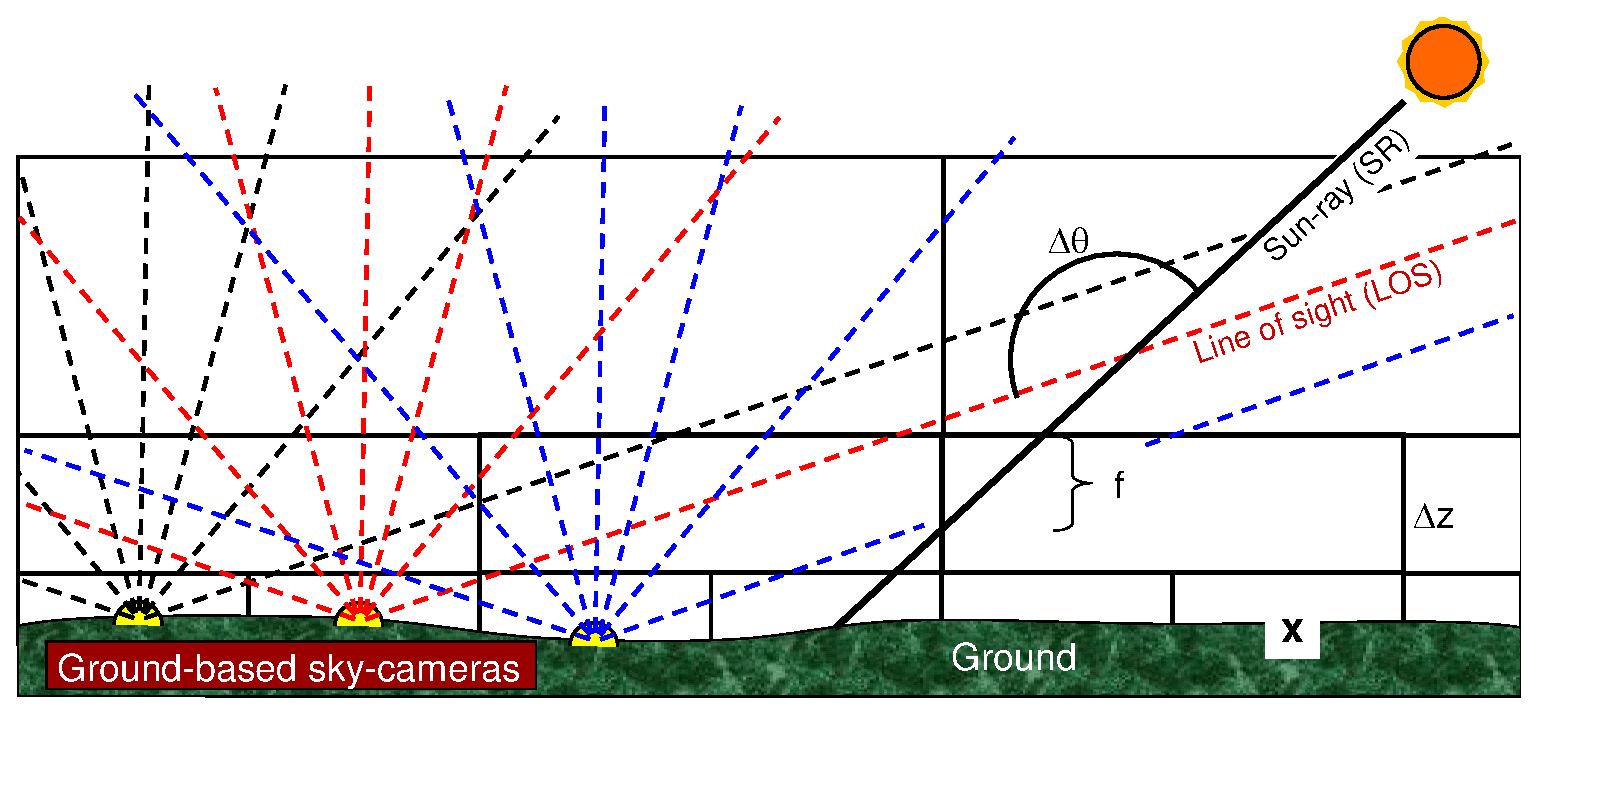
\includegraphics[width=0.99\linewidth]{groundtomog6.eps}
    \end{center}\vspace{-1.5cm}
    \caption{\small
    Lightfield imaging through a volumetric distribution in
    the atmosphere, using ground-based cameras. Our tomographic reconstruction
    follows the acquisition. Irrespective of imaging from space or land, this figure represents the atmosphere in a non-parametric structure, yet the voxel grid gets coarser with altitude, expressing a prior about natural regularity.}
   \label{fig:groundgrid}
\end{figure*}
Ground-based wide-angle sky-cameras capture the sky lightfield from below. Per viewpoint, the view azimuth and elevation angles (relative to the zenith and north) are encapsulated in the vector ${\bf{\Theta}}$.  A raw image is $i_{\bf x}({\bf{\Theta}})$: a camera's location ${\bf x}$ is fixed, while any pixel in a frame represents an angle ${\bf{\Theta}}$.
The measured radiance in all locations ${\bf x}$ and angles ${\bf{\Theta}}$ is the {\em lightfield} $I({\bf x},{\bf{\Theta}})$. Individual images are slices of the lightfield.
 %Alternatively, several ground-based cameras can be mounted on moving vehicles, assuming that the aerosol distribution does not change much during the time-lapse of the camera trajectory.

Sunlight is scattered in the medium along the LOS, creating {\em airlight}~\cite{fattal,narasimhan2,Hschechner2,tan}. For each view ${\bf{\Theta}}$ and ground location ${\bf x}$, the airlight is generally different, depending on the distribution of aerosols both along the LOS, and the along the SRs that hit the LOS.
As Fig.~\ref{fig:groundgrid} shows, for different ${\bf x}$ and ${\bf{\Theta}}$, the LOS cuts through a different set of voxels in the atmosphere. Thus, for each view, the radiance scattered from a voxel is attenuated differently, depending on the distribution of aerosols along the LOS~\cite{hansen}.


A forward model takes as input the aerosol distribution, and outputs image captured at different viewpoints. The model calculates radiative transfer, based on fixed parameters as the Sun's characteristics. We use a single scattering model, in which any SR changes direction (scatters) only once on the way to the camera. This model is valid in atmospheres that are not very dense: inside fog and clouds this model does not apply. Under single-scattering approximation, radiative transfer has three steps (Fig.~\ref{fig:settings}):\\

\vspace{-0.35cm}
\noindent
 1. Attenuation of a SR propagating from the top of the atmosphere
  (TOA) to voxel $k$. \\

\vspace{-0.35cm}
\noindent
 2. Light scattering at voxel $k$, towards a camera.\\

\vspace{-0.35cm}
\noindent
 3. Light attenuation on the LOS from voxel $k$ to the camera.

\noindent
Steps 1 and 3 involve the optical depth
along the light path to and from voxel $k$, analyzed in Sec.~\ref{sec:optical-depth}.
Step 2 involves the scattering coefficient at voxel $k$,
described in Sec.~\ref{sec:scattering}.

%The light transfer, $\mathrm{t}(k)$, is calculated per scattering at
%each voxel $k$.  Let the Sun irradiance at the TOA be $\mathrm{L}^{\rm
%  TOA}$.  The overall transmittance multiplied by $\mathrm{L}^{\rm
%  TOA}$ yields the radiance sensed by the camera. The sum of
%contributions from all voxels is the image captured by the camera,
%\begin{align}
%  \mathrm{I}_{\rm camera}=\mathrm{L}^{\rm TOA} \sum_k \mathrm{t}(k).
%  \label{eq:transatsensor}
%\end{align}

\begin{figure}
  \centering \def\svgwidth{0.8\columnwidth}
  \yoavcomment{\input{images/atmo_settings.pdf_tex}}
  \caption[Settings of the atmosphere simulation]{Settings for the
    atmosphere simulation.}
  \label{fig:settings}
\end{figure}

%%%%%%%%%%%%%%%%%%%%%%%%%%%%%%%%%%%%%%%%
\subsection{Optical Depth}
\label{sec:optical-depth}

An infinitesimal volume contains aerosols. The extinction and scattering coefficients due to aerosols in this volume are, respectively
\begin{equation}
  \beta^{\rm aerosol}=\sigma^{\rm aerosol} n^{\rm aerosol}
  \;\;,\;\;
  \alpha^{\rm aerosol}=\varpi^{\rm aerosol} \beta^{\rm aerosol}
  \;.
  \label{eq:betaer}
\end{equation}
In addition, the infinitesimal volume contain also air molecules. Hence, the overall
extinction and scattering coefficients in this small volume are, respectively
\begin{equation}
  \beta=\beta^{\rm air}+\beta^{\rm aerosol}
  \;\;,\;\;
  \alpha=\alpha^{\rm air}+\alpha^{\rm aerosol}
  \;.
  \label{eq:betair}
\end{equation}

Any voxel generally contains both air molecules and aerosols. Voxels are indexed by $k$ or $q$.
As approximation, assume that within any voxel, the molecular parameters
$\{ \beta^{\rm air}(k),\alpha^{\rm air}(k)\}$ and the aerosol parameters
$\{ \sigma^{\rm aerosol}(k),\varpi^{\rm aerosol}(k), n^{\rm aerosol}(k),g(k)\}$
are constants, e.g., corresponding to the value at each voxel center. These parameters generally change
between voxels.

A voxel's vertical geometric thickness is $\Delta z$.  The Sun zenith angle is $\Phi^{\rm SR}$. Denote a SR line segment between the TOA and the center of voxel $k$ by $[{\rm SR},k]$.
This SR intersects voxel $q$. The geometric length of this intersection
line segment is $\Delta z f_{\rm SR}(q)/\cos\Phi^{\rm SR}$: the factor
\mbox{$f_{\rm SR}(q)\in [0,1]$} expresses how much of the vertical thickness of $q$ is crossed by the SR. Following Eqs.~(\ref{eq:tau},\ref{eq:betair}), the optical depth between the TOA and voxel $k$ is
\begin{equation}
  \tau_{\rm SR}(k)=\frac{1}{\cos\Phi^{\rm SR}}
     \sum_{q \in[{\rm SR},k]}
     \beta(q)\Delta z  f_{\rm SR}(q)
  \;\;.
  \label{eq:lSRn}
\end{equation}
\begin{figure}
  \centering
  \yoavcomment{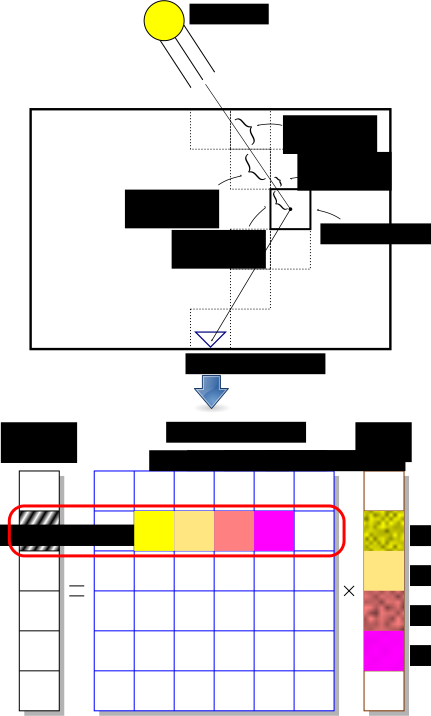
\includegraphics[width=\columnwidth]{images/optical_distance.pdf}}
  \caption{Optical depth calculation}
  \label{fig:optidepth}
\end{figure}
Based on Eqs.~(\ref{eq:betaer},\ref{eq:betair},\ref{eq:lSRn}),
\begin{equation}
  \tau_{\rm SR}(k)=
   \tau_{\rm SR}^{\rm air}(k) +  \tau_{\rm SR}^{\rm aerosol}(k)
  \;\;,
  \label{eq:lSRaa}
\end{equation}
where
\begin{equation}
  \tau_{\rm SR}^{\rm air}(k)=\frac{\Delta z}{\cos\Phi^{\rm SR}}
     \sum_{q \in[{\rm SR},k]}
     \beta^{\rm air}(q)  f_{\rm SR}(q)
  \label{eq:lSRair}
\end{equation}
and
\begin{equation}
  \tau_{\rm SR}^{\rm aerosol}(k)=\frac{\Delta z}{\cos\Phi^{\rm SR}}
     \sum_{q \in[{\rm SR},k]}
     \sigma^{\rm aerosol}(q) n^{\rm aerosol}(q) f_{\rm SR}(q)
  \label{eq:lSRaeros}
\end{equation}

The number of voxels is  $N_{\rm voxels}$. All their associated
variables are concatenated into columns stack vectors, each $N_{\rm voxels}$ long. Aerosol densities and cross sections in all voxels are stored in the respective vectors ${\bf n}$ and $\vect{\sigma}$. Define a $N_{\rm voxels}\times N_{\rm voxels}$ sparse matrix ${\bf D}^{\mathrm{Sun \rightarrow voxel}}$, whose 
element $(k,q)$ is
\begin{equation}
  D^{\mathrm{Sun \rightarrow voxel}}(k,q) =
  \left\{
      \begin{array}{ll}
          \frac{\Delta zf_{\rm SR}(q)}{\cos\Phi^{\rm SR}}
                & \mbox{ if $q \in[{\rm SR},k]$} \\
          0  & \mbox{ otherwise}
    \label{eq:Dsv}
       \end{array}
  \right.
  .
  \hspace{-0.05cm}
\end{equation}
Eqs.~(\ref{eq:lSRaeros},\ref{eq:Dsv}) lead to a vector of SR optical depths due to aerosols:
\begin{equation}
  \vect{\tau}_{\rm SR}^{\rm aerosol}=
  {\bf D}^{\mathrm{Sun \rightarrow voxel}}
     (\vect{\sigma} \odot {\bf n})
  \label{eq:tauSRvec1}
\end{equation}
where the operator $\odot$ denotes the Hadamard (element-wise)
product. 
Similarly, Eq.~(\ref{eq:lSRair}) leads to a vector of SR optical depths due to air,
$\vect{\tau}_{\rm SR}^{\rm air}$.


Analogously, for camera $c$, denote by $[{\rm LOS}_c,k]$
a LOS bounded between the camera and the center of voxel $k$. The LOS zenith angle is $\Phi^{\rm LOS}_c$.
This LOS intersects voxel $q$. The geometric length of this intersection
line segment is $\Delta z f_{\rm LOS_c}(q)/\cos\Phi^{\rm LOS}_c$: the factor
$f_{\rm LOS_c}(q)\in [0,1]$ expresses how much of the vertical thickness of $q$ is crossed by the LOS.
Analogously to Eqs.~(\ref{eq:lSRaa},\ref{eq:lSRair},\ref{eq:lSRaeros}),
The optical depth %path length
along a LOS to $k$ is
\begin{equation}
  \tau_{{\rm LOS}_c}(k)=
   \tau_{{\rm LOS}_c}^{\rm air}(k) +  \tau_{{\rm LOS}_c}^{\rm aerosol}(k)
  \;\;,
  \label{eq:lLOSaerot}
\end{equation}
where
\begin{equation}
  \tau_{{\rm LOS}_c}^{\rm air}(k)=\frac{\Delta z}{\cos\Phi^{\rm LOS}_c}
     \sum_{q \in[{\rm LOS}_c,k]}
     \beta^{\rm air}(q)  f_{\rm LOS_c}(q)
  \label{eq:lLOSair}
\end{equation}
and
\begin{align}
  \label{eq:lLOSaeros}
  \tau_{{\rm LOS}_c}^{\rm aerosol}(k)=
  ~~~~~~~~~~~~~~~~~~~~~~~~~~~~~~~~~~~~~
  ~~~~~~~~~~~~~~~~~~%\nonumber
  ~~~~~
  \\
  %~~~~
   \frac{\Delta z}{\cos\Phi^{\rm LOS}_c}
     \sum_{q \in[{\rm LOS}_c,k]}
     \sigma^{\rm aerosol}(q) n^{\rm aerosol}(q) f_{\rm LOS_c}(q).
     \nonumber
\end{align}
Eq.~(\ref{eq:lLOSaeros}) leads to a vector of LOS optical depths due to aerosols:
\begin{equation}
  \vect{\tau}_{{\rm LOS}_c}^{\rm aerosol}=
  {\bf D}^{\mathrm{voxel \rightarrow cam}}_c
     (\vect{\sigma} \odot {\bf n})
  \label{eq:tauLOSvec1}
\end{equation}
Here ${\bf D}^{\mathrm{voxel \rightarrow cam}}_c$ is a 
$N_{\rm voxels}\times N_{\rm voxels}$ sparse matrix whose element $(k,q)$ is
\begin{equation}
  D^{\mathrm{voxel \rightarrow cam}}_c(k,q) =
  \left\{
      \begin{array}{ll}
          \frac{\Delta z f_{\rm LOS_c}(q)}{\cos\Phi^{\rm LOS}_c}
                & \mbox{ if $q \in[{\rm LOS}_c,k]$} \\
          0  & \mbox{ otherwise}
    \label{eq:Dvc}
       \end{array}
  \right.
  .
  \hspace{-0.05cm}
\end{equation}
%The non-zero elements of the sparse matrix ${\bf D}^{\mathrm{voxel \rightarrow cam}}_c$
%represent $[\Delta z/\cos\Phi^{\rm LOS}_c]f_{\rm LOS_c}(q)$,
%\mbox{$\forall q \in[{\rm LOS}_c,k],$} $\forall k$.
Similarly, Eq.~(\ref{eq:lSRair}) leads to a vector of LOS optical depths due to air,
$\vect{\tau}_{{\rm LOS}_c}^{\rm air}$.

The fixed sparse matrices ${\bf D}^{\mathrm{Sun \rightarrow voxel}}$ and
${\bf D}^{\mathrm{voxel \rightarrow cam}}_c$ are compounded to a single matrix
\begin{equation}
  {\bf D}_c=
  {\bf D}^{\mathrm{Sun \rightarrow voxel}}+
  {\bf D}^{\mathrm{voxel \rightarrow cam}}_c
  \;\;.
  \label{eq:Dtotal}
\end{equation}
Similarly, the molecular optical depths along all trajectories between the sun, each voxel
and camera $c$ are compounded to a vector
\begin{equation}
  \vect{\tau}_c^{\rm air}=
  \vect{\tau}_{\rm SR}^{\rm air}+
  \vect{\tau}_{{\rm LOS}_c}^{\rm air}
  \;\;.
  \label{eq:tauairtotal}
\end{equation}
Using Eq.~(\ref{eq:rayleighbeta}) for $\beta^{\rm air}$ in all voxels,
the vector $\vect{\tau}_c^{\rm air}$ is fixed. Thus $\vect{\tau}_c^{\rm air}$ can
be calculated once, per sun zenith angle.

Using Eqs.~(\ref{eq:lSRaa},\ref{eq:tauSRvec1},\ref{eq:lLOSair},\ref{eq:tauLOSvec1},\ref{eq:Dtotal},\ref{eq:tauairtotal}),
The total optical depths corresponding to LOSs (of camera $c$)  and SRs that cross all voxels comprise the vector
\begin{equation}
  \vect{\tau}_c= \vect{\tau}_c^{\rm air}
               + {\bf D}_c (\vect{\sigma} \odot {\bf n})
  \;\;.
  \label{eq:tautotal}
\end{equation}
This vector depends on the variables $\vect{\sigma}$ and ${\bf n}$.

%%%%%%%%%%%%%%%%%%%%%%%%%%%%%%%%%%%%%%%
\subsection{Scattering}
\label{sec:scattering}

Per camera $c$ and voxel $k$, the lines $[{\rm SR},k]$ and $[{\rm LOS}_c,k]$ intersect at a
fixed angle $\Phi^{\rm scatter}_c(k)$, which is pre-calculated.
%Eq.~(\ref{eq:mu})  yields its cosine, $\mu_c(k)$.
Column-stacking all voxels yields the vector representation of all scattering angles in the domain, $\vect{\Phi}^{\rm scatter}_c$ per camera $c$. Similarly, the single-scattering albdeos
$\varpi^{\rm aerosol}$ in all voxels are stacked to vector $\vect{\varpi}$.
Using Eqs.~(\ref{eq:alphabasic},\ref{eq:rayleighP},\ref{eq:betaer},\ref{eq:betair}), the angular scattering coefficients across the domain are expressed in vector form by
\begin{align}
  \tilde{\vect{\alpha}}^{\rm air}_c &=
    \vect{\beta}^{\rm air} \odot P^{\rm air}(\vect{\Phi}^{\rm scatter}_c)   \nonumber \\
  \tilde{\vect{\alpha}}^{\rm aerosol}_c &=
     \vect{\varpi}\odot
     \vect{\sigma} \odot
     {\bf n} \odot
     P^{\rm aerosol}_{\bf g}(\vect{\Phi}^{\rm scatter}_c)
  \label{eq:alpha_matrix}
\end{align}
The vector ${\bf g}$ column-stacks the anisotropy parameter of the phase function, in all voxels. We use this notation, to indicate a parametric phase function as in Eq.~(\ref{eq:aerosol_scatter}).


%%%%%%%%%%%%%%%%%%%%%%%%%%%%%%%%%%%%%%%%%%%%%%%%%%%%%%%%%%%%%%%%
\subsection{Image Capture}
\label{sec:captured-image}

Compounding the attenuation of irradiance along both $[{\rm SR},k]$ and $[{\rm LOS}_c,k]$, and scattering
by voxel $k$ towards the camera (Eqs.~\ref{eq:beer-lambert},\ref{eq:betair},\ref{eq:tautotal}), the radiant power contributed by the voxel is
\begin{equation}
  p_c(k)= L^{\rm TOA}
          [\tilde{\alpha}^{\rm air}_c(k) + \tilde{\alpha}^{\rm aerosol}_c(k)]
          e^{-[\tau_c(k)]}
  \;\;.
  \label{eq:ick}
\end{equation}
A column-stack vector of all voxel contributions is
\begin{equation}
 {\bf p}_c= L^{\rm TOA}
          [\tilde{\vect{\alpha}}^{\rm air}_c + \tilde{\vect{\alpha}}^{\rm aerosol}_c]
           \odot e^{-\vect{\tau}_c}
  \;\;.
  \label{eq:pc}
\end{equation}

A camera pixel collects light from a narrow cone in the atmosphere.
The cone includes some voxels, intersects with some other voxels, and oblivious to all the rest.
\begin{figure}
  \centering
  \yoavcomment{\includegraphics[width=\columnwidth]{images/sensor.pdf}}
  \caption{Camera projection operation}
  \label{fig:projection}
\end{figure}
Thus the measured radiance at a pixel is weighted sum of the power $p_c(k)$ from all voxels: most voxels have null weight, since they fall outside the pixels's conic field of view, while the rest of the voxels are aggregated.

This linear sum is formulated by a matrix operation over ${\bf p}_c$. 
The pixels in the measured image are column-stacked to a vector 
$N_{\rm pix}$ long. It is given by
\begin{equation}
 {\bf i}_c= {\vect{\Pi}}_c{\bf p}_c
  \;\;.
  \label{eq:IcP}
\end{equation}
The $N_{\rm pix}\times N_{\rm voxels}$ sparse matrix ${\vect{\Pi}}_c$  
expresses {\em projection} of light into camera $c$.
For pixel $\Theta$ and voxel $k$, there is an {\em intersection} volume ${\bf V}_c(\Theta,k)$ between the cone volume of the pixel's field of view, and the voxel, as illustrated in Fig.~\ref{fig:projection}. The corresponding element in the matrix ${\vect{\Pi}}_c$ can be written as
\begin{equation}
 \Pi_c(\Theta,k)=({\rm NA})^2
     \iiint_{{\bf V}_c(\Theta,k)}
     \frac{1}{[R({\bf v})]^2} d{\bf v}
  \;\;,
  \label{eq:Pc}
\end{equation}
where ${\rm NA}$ is the numerical aperture of the camera lens. The distance $R({\bf v})$ is measured between the camera and an infinitesimal volume element at ${\bf v}\in {\bf V}_c(\Theta,k)$.

Combining Eqs.~(\ref{eq:tautotal},\ref{eq:pc},\ref{eq:IcP}), the captured image is thus
\begin{align}
 {\bf i}_c= L^{\rm TOA}
    {\vect{\Pi}}_c
          \left\{
          (\tilde{\vect{\alpha}}^{\rm air}_c + \tilde{\vect{\alpha}}^{\rm aerosol}_c)
           \odot
            e^{-[\vect{\tau}_c^{\rm air}
               + {\bf D}_c (\vect{\sigma} \odot {\bf n})]}
           \right\}
  \label{eq:bigIc}
\end{align}
Most often, there is only a single type of aerosol over a scene. Hence, the three-element
vector $[{\sigma}^{\rm aerosol},\varpi^{\rm aerosol},g]$ is uniform across the scene, but the density distribution ${\bf n}$ is variable. Then, Eq.~(\ref{eq:bigIc}) degenerates to
\begin{align}
 {\bf i}_c= L^{\rm TOA}
    {\vect{\Pi}}_c
          \Big\{
            e^{-(\vect{\tau}_c^{\rm air}
                  + {\sigma}^{\rm aerosol} {\bf D}_c {\bf n})
              }\odot
  \;\;\;\;\;\;\;\;\;\;\;\;\;\;\;\;\;\;\;\;\;
     \nonumber \\
           [\tilde{\vect{\alpha}}^{\rm air}_c + %\right.
           \varpi^{\rm aerosol}\sigma^{\rm aerosol}
           P^{\rm aerosol}_g(\vect{\Phi}^{\rm scatter}_c)
           \odot{\bf n}
           ]
           \Big\}
           .
  \label{eq:bigIA}
\end{align}


%%%%%%%%%%%%%%%%%%%%%%%%%%%%%%%%%%%%%%%%%%%%%%%%%%%%%%%%%%%
\section{Inverse Problem}
\label{sec:inverse-problem}

%%%%%%%%%%%%%%%%%%%%%%%%%%%%%%%%%%%%%%%%%%%%%%%%%%%%%%%%%%%
\subsection{Unknowns and Prior Knowledge}
\label{sec:prior}

In general terms, the variables are the set
\begin{equation}
 {\cal V}\equiv
  \left\{
    {\bf n},
     \left\{
       \vect{\varpi}_{\lambda},\vect{\sigma}^{\rm aerosol}_{\lambda},{\bf g}_{\lambda}
      \right\}_{\lambda}
   \right\}
  \;\;,
  \label{eq:calV}
\end{equation}
where $\lambda$ denotes the spectral (color) channel. 
There are $N_{\rm spectral}$ spectral channels. 
Thus, the number of unknown variables is in principle \mbox{$|{\cal V}|=N_{\rm voxels}(1+3N_{\rm spectral})$}.


Prior knowledge reduces the unknowns. Sec.~\ref{sec:captured-image} mentions a prior:
in many cases a single aerosol type dominates a scene. Then, the three-element
vector $[\varpi,{\sigma}^{\rm aerosol},g]$ is rather spatially uniform. In such cases, the set of unknowns
reduces to
$ {\cal V}=
  \left\{
    {\bf n},
     \left\{
       {\varpi}_{\lambda},{\sigma}^{\rm aerosol}_{\lambda},g_{\lambda}
      \right\}_{\lambda}
   \right\}
$
and \mbox{$|{\cal V}|=N_{\rm voxels}+3N_{\rm spectral}$}.

Furthermore, the elements in the aerosol characteristics
set $\left\{
       {\varpi}_{\lambda},{\sigma}^{\rm aerosol}_{\lambda},g_{\lambda}
      \right\}_{\lambda}$
is not arbitrary, since all these characteristics have physical origins. This
set is constrained to comply with what nature allows (aerosol classes).
This significantly constrains the unknown characteristics. State-of-the-art aerosol retrieval,
as used by NASA's MISR products indeed employ an aerosol-class prior. Types of aerosol mixtures are discretized to $N_{\rm models}=74$ classes~\cite{martonchikBook}, called {\em models}.
Each class $m$ represents aerosols having a distinct characteristics set.
State of the art retrieval is 1D (only vertical radiative transfer per large areas). We use
this prior in our 3D problem. Then, the set of unknowns reduces to
$ {\cal V}= \left\{ {\bf n},m  \right\}$
and \mbox{$|{\cal V}|=N_{\rm voxels}+N_{\rm models}$}.

The atmosphere is photographed from $N_{\rm views}$ viewpoints. Each photograph provides $N_{\rm pix}$  measurements (pixels), {\em including} their possible division to color channels. Hence, the data at our disposal comprises $N_{\rm views}N_{\rm pix}$ measurements.
For the recovery task to be well-posed, it is necessary that 
$N_{\rm views}N_{\rm pix}>|{\cal V}|$.


%%%%%%%%%%%%%%%%%%%%%%%%%%%%%%%%%%%%%%%%%%%%%%%%%%%%%%%%%%%
\subsection{Objective Function}
\label{sec:objective-function}

The inverse problem (tomography) seeks recovery of the 3D aerosol distribution in the atmosphere. From Eqs.~(\ref{eq:alpha_matrix},\ref{eq:bigIc},\ref{eq:bigIA},\ref{eq:calV}),
the images $\{ {\bf i}_c\}_{c=1}^{N_{\rm views}}$ depend on the variables set ${\cal V}$, particularly on the unknown field ${\bf n}$. The recovery task is phrased as optimization of an objective function, that fits the image-formation model~(\ref{eq:bigIc},\ref{eq:bigIA}) to
measured photographs $\{ {\bf i}^{\rm measured}_c\}_{c=1}^{N_{\rm views}}$:
\begin{equation}
  \label{eq:mingenobjective}
  \hat{\cal V} = \argmin_{{\cal V}\in {\cal C}} f({\cal V})
\end{equation}
where
\begin{equation}
  \label{eq:genobjective}
  f({\cal V}) = \sum_{c=1}^{N_{\rm views}}
  \| {\bf i}^{\rm measured}_c - {\bf i}_c({\cal V})\| + {\rm Regularization}({\cal V})
  \;.
\end{equation}
Here ${\cal C}$ is a constraints set, which encapsulates part of the prior knowledge,
as well as nonnegativity bounds, while $\|~\|$ is some error-distance measure.
Here ${\rm Regularization}({\cal V})$ describes spatial regularization terms of the variables, such as smoothness, a blobby or a layered structure.

Spatial regularization can help overcome lack of data, if $N_{\rm views}$ is too small, and it is definitely helpful. In this work, however, we formulate and demonstrate the basic principle of our tomography task, hence
we proceed without regularization. Relying on prior knowledge described in Sec.~\ref{sec:prior}, the problem complexity is by far dominated by the $N_{\rm voxels}$-large array ${\bf n}$, which is continuously valued. Hence, we focus here on retrieving ${\bf n}$ through continuous optimization. Relying on the mean-squared error measure, we seek:
\begin{equation}
  \label{eq:minobjectiveA}
  \hat{\bf n} =
      \argmin_{{\bf n}} f({\bf n})
\end{equation}
where
\begin{equation}
  \label{eq:objectiveA}
  f({\bf n})
   = \sum_{c=1}^{N_{\rm views}}
  \| {\bf i}^{\rm measured}_c - {\bf i}_c({\bf n})\|^2_2
\end{equation}
This is solved using standard optimization tools. Fast optimization that leads to
to local minima ($f$ is not convex) exploits the gradient of $f$.

Since our model uses close-form expressions, $f$ is differentiable. The gradient of $f$ with respect to ${\bf n}$ is
\begin{align}
  \Grad{{\bf n}} f = -2\sum_{c=1}^{N_{\rm views}}
  \transpose{\left[{\bf J}_{{\bf i}_c}({\bf n})\right]}
  [{\bf i}^{\rm measured}_c - {\bf i}_c({\bf n})]
  \;.
  \label{eq:gradient1}
\end{align}
Here the matrix ${\bf J}_{{\bf i}_c}({\bf n})$ is the Jacobian  of
the vector ${\bf i}_c$ with respect to ${\bf n}$. Element $(\Theta,k)$ of this matrix
differentiates the intensity in pixel ${\bf \Theta}$ (in viewpoint $c$) with variation of the density at voxel $k$, i.e.,
  $\partial i_c({\bf \Theta})/\partial{n^{\rm aerosol}(k)}$.

Denote by $\OpDiag{\vect{v}}$ conversion of vector $\vect{v}$ into a diagonal matrix, whose main diagonal elements correspond to the elements of $\vect{v}$.
A close-form expression of the Jacobian is
\begin{align}
  {\bf J}_{{\bf i}_c}({\bf n}) &= 
    L^{\rm TOA}({\bf A}-{\bf B}){\bf C} ,
  \label{eq:gradient2}
\end{align}
where
\begin{align}
  \label{eq:gradient3}
  {\bf A} &= 
    \varpi^{\rm aerosol}\sigma^{\rm aerosol}
         \OpDiag{ P_g^{\rm aerosol}(\vect{\Phi}^{\rm scatter}_c)} \nonumber\\
 {\bf B} &= {\sigma}^{\rm aerosol}\transpose{{\bf D}_c} \nonumber\\
       & \;\;\;
       \OpDiag{[\tilde{\vect{\alpha}}^{\rm air}_c 
                + \varpi^{\rm aerosol}\sigma^{\rm aerosol} 
                P^{\rm aerosol}_g(\vect{\Phi}^{\rm scatter}_c) \odot{\bf n}
                ]} \nonumber \\
  {\bf C} &= \OpDiag{\exp[-(\vect{\tau}_c^{\rm air} 
          + {\sigma}^{\rm aerosol} {\bf D}_c {\bf n})]} 
          \transpose{{\vect{\Pi}}_c}
\end{align}
For a detailed derivation of Eqs.~(\ref{eq:gradient2},\ref{eq:gradient3}),
we refer the reader to the supplementary material.



%%%%%%%%%%%%%%%%%%%%%%%%%%%%%%%%%%%%%%%%%%%%%%%
\section{Simulations}
\label{sec:simul}



To test the model, we made simulations based on atmospheric models in the literature. Here are the details.\\

\noindent{\bf Sun}: The sun is at zenith angle $\Phi^{\rm SR}=45^o$. Its
$L^{\rm TOA}$ is obtained from~\cite{BBradiance,sun_composition}, with respective red-green-blue ratios of
 $L^{\rm TOA}_{\rm R}:L^{\rm TOA}_{\rm G}:L^{\rm TOA}_{\rm B}=255:236:224$.\\

\noindent{\bf Aerosol}: We used particle-type 6 from the aerosol list in
Ref.~\cite{Martonchik2009}. This is a spherical non-absorbing sea-salt/organic particle, whose anisotropy parameter per color channel is $[g_{\rm R},g_{\rm G},g_{\rm B}]=[0.763,0.775,0.786]$. Its corresponding extinction cross sections are
  $[\sigma^{\rm aerosol}_{\rm R},
    \sigma^{\rm aerosol}_{\rm G},
    \sigma^{\rm aerosol}_{\rm B}]=[16.5,16.2,15.9][1/\mu m^2]$.
Its single-scattering albedo is $\varpi^{\rm aerosol}=1$ at all channels.
We set the spatial distribution as a product of two functions. The first function is an exponential decay~\cite{Levi1980} with altitude $h(k)$ of voxel $k$,
\begin{align}
 w_1[h(k)] = \frac{1}
 {\sigma^{\rm aerosol}_{\rm G} \mathrm{MFP^{sea level}}}
  \exp\left[-\frac{h(k)}{H^\mathrm{aerosol}}\right],
\end{align}
where $H^\mathrm{aerosol}=2\ km$. This expresses a general trend of reduced atmospheric density with height. Here
The mean free path (MFP) of the aerosols layer at sea level is
$\mathrm{MFP^{sea level}}=1/5~{\rm[1/km]}$.
% is a typical characteristic thickness of the aerosol layer~\cite{Levi1980}.

The second function, $w_2$, expresses a clustered nature of aerosol ``clouds''. We define two ellipsoids: the first is centered at altitude
$3.3km$, and has horizontal width of $32km$ and vertical thickness of $2.8km$. The second ellipsoid is centered at altitude $6.6km$, and has lateral width of $24km$ and vertical thickness of $2.1km$. Then
\begin{equation}
  w_2(k) =
  \left\{
      \begin{array}{ll}
          1  & \mbox{ if $k\in$ any ellipsoid} \\
          0  & \mbox{ otherwise}
    \label{eq:f2}
       \end{array}
  \right.
  .
  \hspace{-0.05cm}
\end{equation}
The aerosol distribution is then ${\bf n}={\bf w}_1\odot {\bf w}_2$.
Note that the horizontal widths are much larger than the vertical ones. This is consistent with scales of atmospheric aerosol distributions.\\

\noindent{\bf Dimensions}: The domain of sky we simulate and recover has area of $50\times 50$km, and it extends from the ground up to altitude of 10km. This volume is divided to a $50\times50\times100$ grid, where each voxel has area of $1\times1$km and vertical thickness of 100 meters. The dimension of the problem is thus $250,000$ variables.\\

\noindent{\bf Cameras}: Each ground-based camera has a hemispherical field of view, capturing the entire sky from its viewpoint. We used 95 viewpoints on a grid, each view $\approx 4.4$km from its neighbors.
The resolution of each camera is low: $128\times 128$ pixels, expressing the fact that cloudless (yet hazy) sky images are rather smooth, hence there is no need for high image resolution. Each pixel has full-well depth of 40000 electrons, which corresponds to the brightest pixel value. Each measurement has photon noise, which is Poissonian distributed, according to image value $i_c$ and the full-well depth.\\

\noindent{\bf Computer}: We had access to an SGI-TNN cluster computer that has 88 computer nodes consisting of two 2.40 GHz six-Core Xeon with 8GB
DDR3 memory per core. Out of it, we used 8 nodes, corresponding to 96 cores. Each core was dedicated to rendering a modeled image (in each interaction) as if captured by one of the 95 cameras. Each iteration (varying the model according to the gradient-based algorithm and varying all the rendered images) took $\approx 7$sec.\\

\noindent{\bf Optimization}: We used the L-BFGS-B algorithm~\cite{BFGS}. The algorithm was initialized by ${\bf n}=0$. Satisfactory convergence occurred in several thousand iterations, taking a couple of hours to complete in total.

%26, 48, 1320, 590
%%%%%%%%%%%%%%%%%%%%%%%%%%%%%%%%%%%%%%%%%%%%%%%%%%%
\subsection{Optimization Results}
\label{sec:optimization-results}

Fig.~\ref{fig:simulation-results1} shows two modeled images out of 95 from
created by the `spheres' simulation.
\begin{figure}
  \centering
  \yoavcomment{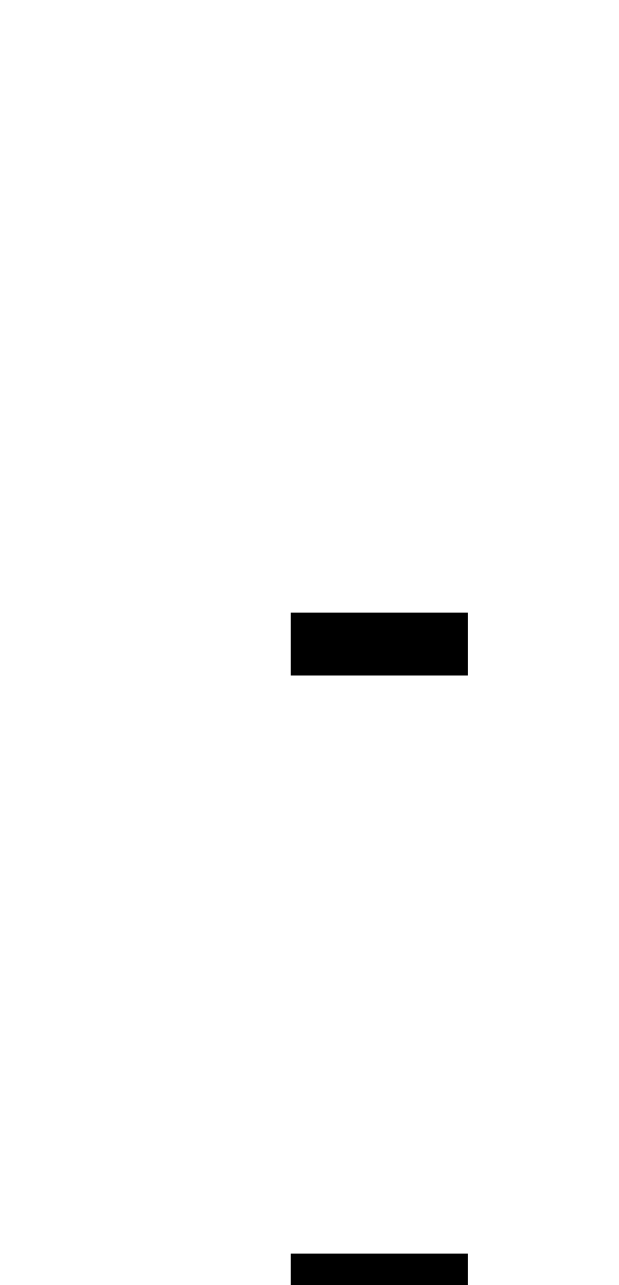
\includegraphics[width=0.8\columnwidth]{images/ref_images.pdf}}
  \caption{Synthesised images taken from different views. A yellow dot marks
    the Sun location. Dashed white circles mark elevation.}
  \label{fig:simulation-results1}
\end{figure}

Fig.~\ref{fig:simulation1} shows an iso-surface visualization of the original
`spheres' distribution and its reconstruction.
\begin{figure}
  \centering
  \yoavcomment{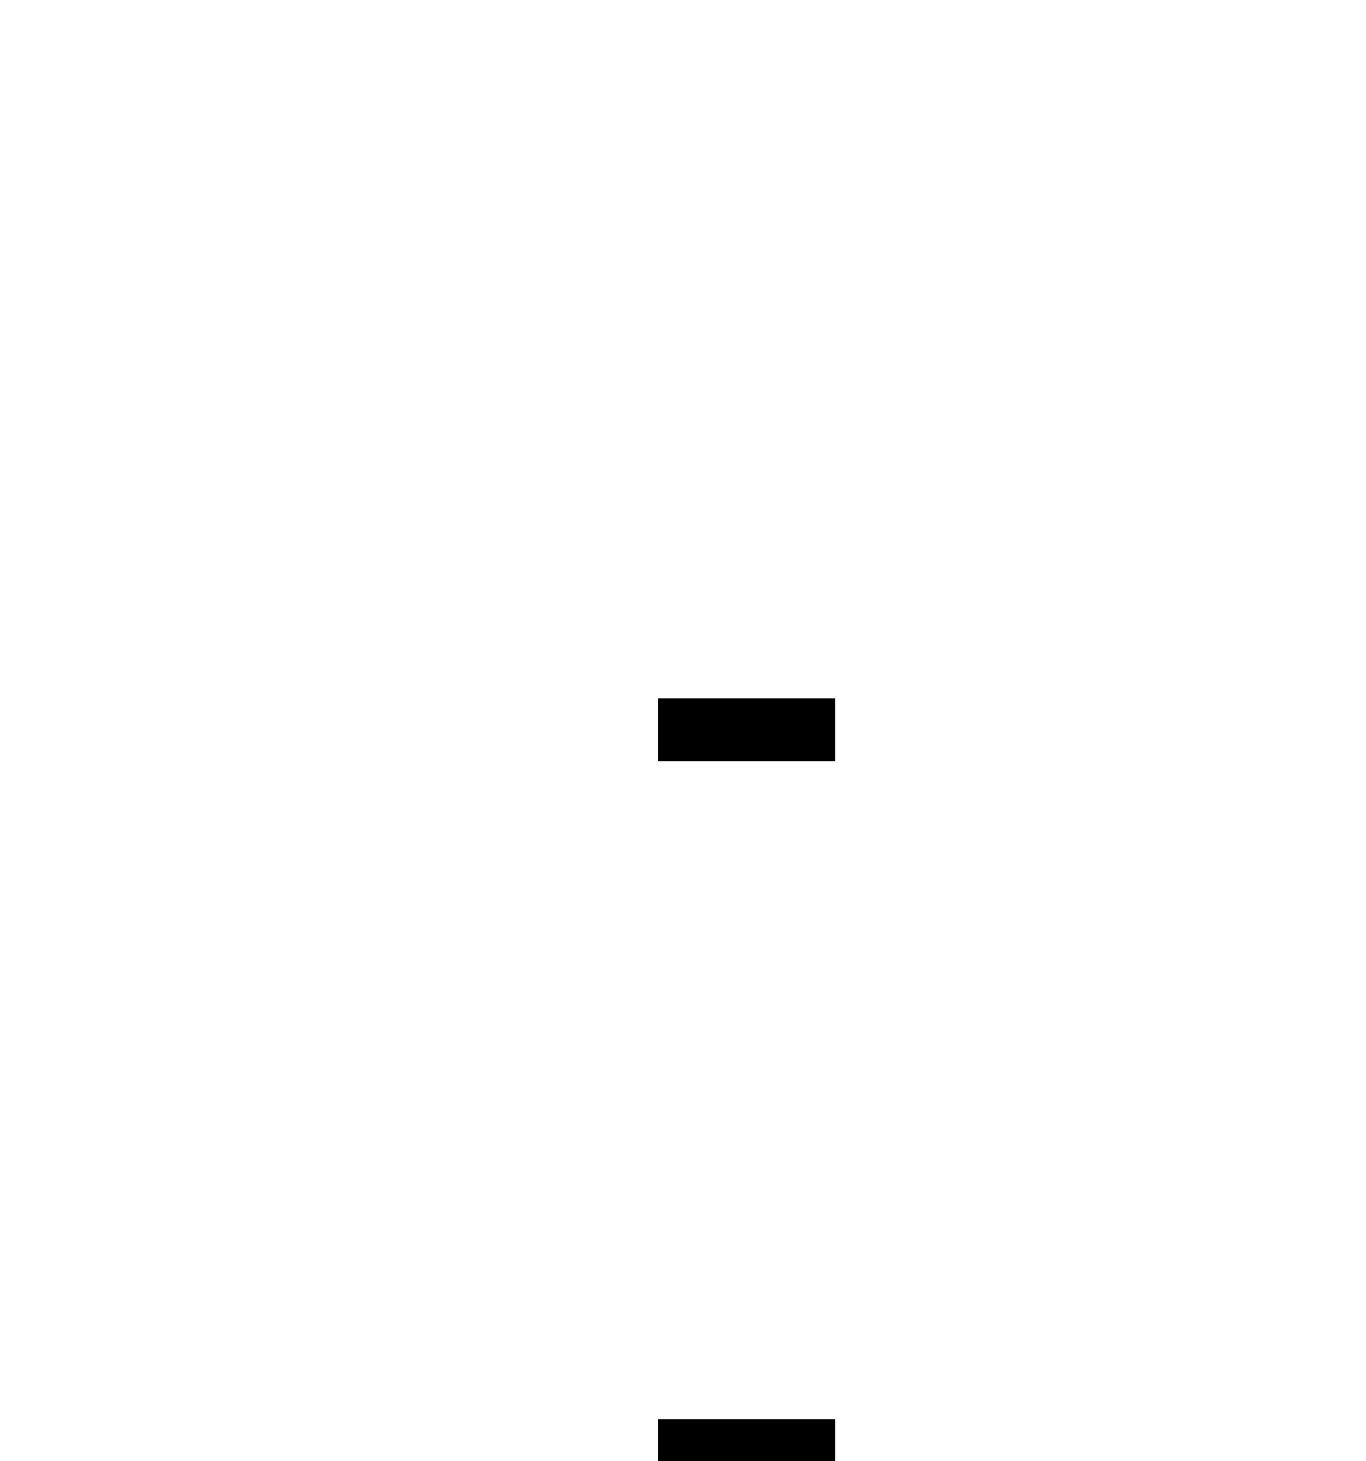
\includegraphics[width=\columnwidth]{images/simulation1}}
  \caption{Synthetic 3D aerosol distribution from the `spheres' simulation (a) and its reconstruction (b). Colour values mark
    aerosol density.}
  \label{fig:simulation1}
\end{figure}

Fig.~\ref{fig:simulation2} shows an iso-surface visualization of the original
`front' distribution and its reconstruction.
\begin{figure}
  \centering
  \yoavcomment{\includegraphics[width=\columnwidth]{images/simulation2}}
  \caption{Synthetic 3D aerosol distribution from the `front' simulation (a) and its reconstruction (b). Colour values mark
    aerosol density.}
  \label{fig:simulation2}
\end{figure}

Fig.~\ref{fig:objective} shows the progression of the objective as a function
of the iteration number. As can be seen by the graph, convergence occurs
after several thousand iteration. 
\begin{figure}[htbp]
  \centering
  \includegraphics[width=\columnwidth]{images/objective.eps}
  \caption{The log of the objective as function of the iteration.}
  \label{fig:objective}
\end{figure}

%%%%%%%%%%%%%%%%%%%%%%%%%%%%%%%%%%%%%%%%%%%%%%%%%%%
\subsection{Conclusions}
\label{sec:conclusions}

{\small
%\bibliographystyle{ieee}
%\bibliography{atmosphere}

\begin{thebibliography}{10}\itemsep=-1pt

\bibitem{baxter}
B.~Baxter, B.~Hooper, J.~Williams, and J.~Dugan.
\newblock Polarimetric remote sensing of ocean waves.
\newblock Proc. MTS/IEEE OCEANS 2009.

\bibitem{bishop}
T.~E. Bishop, S.~Zanetti, and P.~Favaro.
\newblock Light field superresolution.
Proc. IEEE ICCP 2009.

\bibitem{breon}
F.~Br\'{e}on.
\newblock An analytical model for the cloud-free atmosphere/ocean system
  reflectance.
\newblock {\em Remote Sensing of Environment}, 43(2):179 -- 192, 1993.

\bibitem{chang}
G.~C. Chang and R.~W. Gould.
\newblock Comparisons of optical properties of the coastal ocean derived from
  satellite ocean color and in situ measurements.
\newblock {\em Opt. Express}, 14(22):10149--10163, 2006.

\bibitem{BBradiance}
M.~Charity.
\newblock Blackbody color datafile, 2001.
\newblock [Online; accessed 6-August-2012].

\bibitem{chud}
A.~Chudnovsky, A.~Kostinski, L.~Herrmann, I.~Koren, G.~Nutesku, and E.~Ben-Dor.
\newblock Hyperspectral spaceborne imaging of dust-laden flows: Anatomy of
  saharan dust storm from the Bod\'{e}l\'{e} depression.
\newblock {\em Remote Sensing of Environment}, 115(4):1013 -- 1024, 2011.

\bibitem{matronchik}
J.~M. David, D.~J. Diner, R.~Kahn, T.~P. Ackerman, M.~M. Verstraete, B.~Pinty,
  and H.~R. Gordon.
\newblock Techniques for the retrieval of aerosol properties over land and
  ocean using multi-angle imaging.
\newblock {\em IEEE Trans. Geoscience and Remote Sensing},
  36:1212--1227, 1998.

\bibitem{martonchikBook}
J.~M. David, D.~J. Diner, R.~Kahn, T.~P. Ackerman, M.~M. Verstraete, B.~Pinty,
  and H.~R. Gordon.
\newblock Techniques for the retrieval of aerosol properties over land and
  ocean using multi-angle imaging.
\newblock {\em IEEE Trans. Geoscience and Remote Sensing},
  36:1212--1227, 1998.

\bibitem{dayan}
U.~{Dayan}, B.~{Ziv}, T.~{Shoob}, and Y.~{Enzel}.
\newblock {Suspended dust over southeastern Mediterranean and its relation to
  atmospheric circulations}.
\newblock {\em Int. J. Climatology}, 28:915--924, 2008.

\bibitem{dinerDavis10}
D.~J. Diner, A.~Davis, B.~Hancock, S.~Geier, B.~Rheingans, V.~Jovanovic,
  M.~Bull, D.~M. Rider, R.~A. Chipman, A.-B. Mahler, and S.~C. McClain.
\newblock First results from a dual photoelastic-modulator-based polarimetric
  camera.
\newblock {\em Appl. Opt.}, 49(15):2929--2946, 2010.

% \bibitem{dinerDavis07}
% D.~J. Diner, A.~Davis, B.~Hancock, G.~Gutt, R.~A. Chipman, and B.~Cairns.
% \newblock Dual-photoelastic-modulator-based polarimetric imaging concept for
%   aerosol remote sensing.
% \newblock {\em Appl. Opt.}, 46(35):8428--8445,  2007.

\bibitem{diner}
D.~J. Diner and J.~V. Martonchik.
\newblock Atmospheric transmittance from spacecraft using multiple view angle
  imagery.
\newblock {\em Appl. Opt.}, 24(21):3503--3511, 1985.

\bibitem{fattal}
R.~Fattal.
\newblock Single image dehazing.
\newblock In {\em ACM SIGGRAPH}, 72:1--72:9, 2008.

\bibitem{fuchs}
C.~Fuchs, M.~Heinz, M.~Levoy, H.-P. Seidel, and H.~P.~A. Lensch.
\newblock Combining confocal imaging and descattering.
\newblock {\em Computer Graphics Forum}, 27(4):1245--1253, 2008.

\bibitem{gorbunov}
M.~Gorbunov, S.~Sokolovsky, L.~Bengtsson, %and M.-P.-I. f{\"u}r Meteorologie.
\newblock {\em Space Refractive Tomography of the Atmosphere: Modeling of
  Direct and Inverse Problems}.
\newblock Max-Planck-Institut f{\"u}r Meteorologie report, 1996.

\bibitem{gregson}
J.~Gregson, M.~Krimerman, M.~B. Hullin, and W.~Heidrich.
\newblock Stochastic tomography and its applications in 3d imaging of mixing
  fluids.
\newblock {\em ACM TOG}, 31(4):52:1--52:10, 2012.

\bibitem{hansen}
J.~Hansen and L.~Travis.
\newblock Light scattering in planetary atmospheres.
\newblock {\em Space Science Reviews}, 16:527--610, 1974.

\bibitem{he}
K.~He, J.~Sun, and X.~Tang.
\newblock Single image haze removal using dark channel prior.
\newblock {\em IEEE Trans. PAMI}, 33(12):2341 --2353, 2011.

\bibitem{horstmeyer}
R.~Horstmeyer, G.~Euliss, R.~Athale, and M.~Levoy.
\newblock Flexible multimodal camera using a light field architecture.
\newblock Proc. IEEE ICCP, 2009.

\bibitem{ihrke}
I.~Ihrke, K.~N. Kutulakos, H.~P.~A. Lensch, M.~Magnor, and W.~Heidrich.
\newblock State of the art in transparent and specular object reconstruction,
  2008.

\bibitem{johnsen}
S.~Johnsen and H.~M. Sosik.
\newblock Shedding light on light in the ocean.
\newblock {\em Oceanus}, 43:24--28, 2004.

\bibitem{kalashnikova}
O.~V. Kalashnikova, M.~J. Garay, A.~B. Davis, D.~J. Diner, and J.~V.
  Martonchik.
\newblock Sensitivity of multi-angle photo-polarimetry to vertical layering and
  mixing of absorbing aerosols: Quantifying measurement uncertainties.
\newblock {\em J. Quantitative Spectroscopy and Radiative Transfer},
  112(13):2149 -- 2163, 2011.

\bibitem{kim}
J.~Kim, D.~Lanman, Y.~Mukaigawa, and R.~Raskar.
\newblock Descattering transmission via angular filtering.
\newblock In. Proc. ECCV, 86--99, 2010.

\bibitem{kokhan}
A.~Kokhanovsky.
\newblock {\em Light Scattering Media Optics}.
\newblock Springer Praxis Books / Environmental Sciences, 2005.

\bibitem{kopf}
J.~Kopf, B.~Neubert, B.~Chen, M.~F. Cohen, D.~Cohen-Or, O.~Deussen,
  M.~Uyttendaele, and D.~Lischinski.
\newblock Deep photo: Model-based photograph enhancement and viewing.
\newblock {\em ACM TOG}, 27(5):116:1--116:10, 2008.

\bibitem{kratz}
L.~Kratz and K.~Nishino.
\newblock Factorizing scene albedo and depth from a single foggy image.
\newblock In {\em Proc. IEEE ICCV}, 2009.

\bibitem{Levi1980}
L.~Levi.
\newblock {\em Applied Optics}, volume~2.
\newblock Jhon Wiley \& Sons, Inc, 1980.

\bibitem{levoy}
M.~Levoy, B.~Chen, V.~Vaish, M.~Horowitz, I.~McDowall, and M.~Bolas.
\newblock Synthetic aperture confocal imaging.
\newblock {\em ACM TOG}, 23(3):825--834, Aug. 2004.

\bibitem{levy}
M.~Levy, Y.~Lehahn, J.-M. Andre, L.~Memery, H.~Loisel, and E.~Heifetz.
\newblock {Production regimes in the northeast Atlantic: A study based on
  Sea-viewing Wide Field-of-view Sensor (SeaWiFS) chlorophyll and ocean general
  circulation model mixed layer depth}.
\newblock {\em J. Geophys. Res.}, 110(C7):C07S10, 2005.

\bibitem{Martonchik2009}
J.~V. Martonchik, R.~A. Kahn, and D.~J. Diner.
\newblock {Retrieval of aerosol properties over land using MISR observations}.
\newblock In A.~A. Kokhanovsky and G.~Leeuw, editors, {\em Satellite Aerosol
  Remote Sensing over Land}, pages 267--293, Springer Praxis Books,
  Berlin 2009.

\bibitem{messer}
H.~Messer, A.~Zinevich, and P.~Alpert.
\newblock Environmental sensor networks using existing wireless communication
  systems for rainfall and wind velocity measurements.
\newblock {\em IEEE Instrumentation Measurement Magazine}, 15(2):32 --38,
  2012.

\bibitem{moses}
W.~J. Moses, A.~A. Gitelson, S.~Berdnikov, and V.~Povazhnyy.
\newblock Estimation of chlorophyll- a concentration in case ii waters using
  modis and meris data-successes and challenges.
\newblock {\em Environmental Research Letters}, 4(4):045005, 2009.

\bibitem{narasimhan2}
S.~G. Narasimhan and S.~K. Nayar.
\newblock Vision and the atmosphere.
\newblock {\em Int. J. Comput. Vision}, 48(3):233--254,  2002.

\bibitem{oakley}
J.~P. Oakley and B.~L. Satherley.
\newblock Improving image quality in poor visibility conditions using a
  physical model for contrast degradation.
\newblock {\em Trans. Img. Proc.}, 7(2):167--179, 1998.

\bibitem{Hschechner2}
Y.~Y. Schechner, S.~G. Narasimhan, and S.~K. Nayar.
\newblock Polarization-based vision through haze.
\newblock {\em Appl. Opt.}, 42(3):511--525, 2003.

\bibitem{tan}
R.~Tan.
\newblock Visibility in bad weather from a single image.
\newblock In {\em Proc. IEEE CVPR}, 2008.

\bibitem{vanMol}
B.~van Mol and K.Ruddick.
\newblock The compact high resolution imaging spectrometer (CHRIS): the future
  of hyperspectral satellite sensors.
\newblock {\em Airborne Imaging Spectros. Worksh.}, 2004.

\bibitem{sun_composition}
Wikipedia.
\newblock Sunlight --- wikipedia{,} the free encyclopedia, 2012.
\newblock [Online; accessed 6-August-2012].

\bibitem{wright}
T.~E. Wright, M.~Burton, D.~M. Pyle, and T.~Caltabiano.
\newblock {Scanning tomography of SO2 distribution in a volcanic gas plume}.
\newblock {\em Geophys. Res. Lett.}, 35(17):L17811, 2008.

\bibitem{BFGS}
C.~Zhu, R.~H. Byrd, P.~Lu, and J.~Nocedal.
\newblock Algorithm 778: L-BFGS-B: Fortran subroutines for large-scale
  bound-constrained optimization.
\newblock {\em ACM Trans. Math. Softw.}, 23(4):550--560, Dec. 1997.

\end{thebibliography}



}

\end{document}
